% 英文で執筆する場合はクラスファイルへのオプションを[T,E]としてください.
% If you want to write your paper in English, pass to [T,E] options to document class.
\documentclass[T,J]{fose} % 「コンピュータソフトウェア」用のクラスファイルは compsoft です.
\taikai{2024} % 固定です.出版委員長が毎年変更してAuthor Kitを配布してください.

\usepackage [dvipdfmx] {graphicx}

% ユーザが定義したマクロなどはここに置く.ただし学会誌のスタイルの
% 再定義は原則として避けること.

% 以下は説明のために使用したパッケージであるため,削除可能.
\usepackage{listings}
\usepackage{tabularx}
\usepackage{fancyvrb}
\usepackage{xurl}
\usepackage{cite}
\usepackage[dvipdfmx]{graphicx}
\usepackage{latexsym}
\usepackage[T1]{fontenc}
\usepackage{lmodern}
\usepackage{textcomp}
\usepackage{latexsym}
\usepackage{url}
%\usepackage[noadjust]{cite}

\newcommand{\todo}[1]{\colorbox{yellow}{{\bf TODO}:}{\color{red} {\textbf{[#1]}}}}
\newcommand{\rqone}{リリースまでの期間に応じた変更提案の特徴は異なるのか?}
\newcommand{\rqtwo}{変更提案の特徴に基づき,直近のリリースに導入される変更提案をどの程度予測できるのか?}
\newcommand{\rqthree}{優先的に検証される特徴を持つ変更提案のうち,開発者が検証可能と示唆される変更提案は価値があるのか?}

% 以下のマクロはサンプルファイル作成用のマクロです.不要であれば削除してください.
\newcommand{\foseclassfile}{fose.cls}
\newcommand{\fosestylefile}{fose.sty}


\begin{document}

% 論文のタイトル
\title{タイトル}
% 以下の \etitle(と\@etitle)はFOSE論文フォーマット独自のマクロです.
% FOSEに投稿した論文を発展させてコンピュータソフトウェアに投稿される場合はコメントアウトしてください.
% \setetitleは奇数ページのヘッダに表示する文字列(\etitle)を設定するためのマクロです.
% タイトルが2行に渡る場合は "\\" を 使用することで任意の位置で改行をすることができます.
\setetitle{title}
%\setetitle{Long Long Long Long Long Long \\ Long Long Long Long Long \\ Long Long Long Long Long Long Long Long Long Long Long Long Paper Title}

% タイトル,著者などが複数行にわたり,論文冒頭の著者名が日本語アブストと重複して描画された場合に以下のコメントアウトを外してください.
%\longtitle

% 著者
% 和文論文の場合,姓と名の間には半角スペースを入れ,
% 複数の著者の間は全角スペースで区切る
%
\author{上中 瑞稀 伊原 彰紀 大平 雅雄
%
% ここにタイトル英訳 (英文の場合は和訳) を書く.
% 英語タイトルは論文1ページ目左下,著者らの名前・所属一覧の一番上に表示される
%
% 上記\setetitle中で改行した場合は "\etitle" を削除し,改行(\\)を入れていないタイトルを記載してください.
% \ejtitleは1ページ目左下に挿入されるタイトルとして使用されます.
% また,"\etitle"はFOSE論文フォーマット独自のマクロです.
\ejtitle{\etitle}
\shozoku{Mizuki Uenaka, Akinori Ihara, Masao Ohira}{和歌山大学}
{Wakayama University}
}

%
% 和文アブストラクト
% In English paper, content of Jabstract will be ignored. 
\Jabstract{%
本稿はソフトウェア工学の基礎ワークショップのために,実践的IT教育シンポジウム rePiTの論文執筆キットおよび第29回ソフトウェア工学の基礎ワークショップの論文執筆キットを基に作成したものです.
rePiTの論文執筆キットはそもそもソフトウェア科学会の論文執筆キットを基に作成したものです.
具体的な変更箇所は\ref{sec:PaperStyle}章をご参照ください.}
%
% 英文アブストラクト(本サンプルの原論文にはなし)
\Eabstract{
This document has been prepared as a sample for FOSE(Foundation of Software Engineering) based on the Author Kit for rePiT and FOSE2022.
The author kit for rePiT was originally based on author kit of JSSST Computer Software.
The detail changes are written in Sec.\ref{sec:PaperStyle}
}
%
\maketitle \thispagestyle {empty}
\section{はじめに}
ソフトウェア開発において,変更提案されたソースコードの可読性や欠陥の有無を開発者が評価するコードレビューの作業は,ソフトウェアの品質維持のために重要な役割を担っている~\cite{quality1}\cite{quality2}.コードレビューでは,複数人の開発者(検証者)がソースコードを検証し,ソースコードを実装した開発者(実装者)とソースコード変更の妥当性の合意形成を図り,必要に応じて修正を繰り返す.したがって,ソフトウェア開発プロセスの一連の作業において,コードレビューは時間,作業量ともに高いコストを要する作業となっている\cite{cost}.

コードレビューを効率化するため,昨今では多くのソフトウェア開発においてGitHub,Gerrit,Review Boardなどのオンラインコードレビューサービスを利用したコードレビュー方式(モダンコードレビュー\cite{quality1})を導入している.
日々膨大なソースコードの変更提案が提出されるため,検証者は変更提案の内容や緊急性を考慮して,優先的に検証する変更提案を選択している\cite{}.
%引用ほしい
%検証者は直近にリリースするバージョンに導入する変更提案としてソフトウェアの脆弱性を解決する変更提案などを優先して検証する.¥todo{}
%引用ほしい

従来研究では,機械学習アルゴリズムを用いて主に変更提案の提出時に得られる特徴(変更行数や変更ファイル数など)に基づき,翌日までに検証される変更提案を予測する手法を提案している\cite{prioritizer}.この従来研究では,個々の変更提案に対する開発者の関心,変更提案をソフトウェアに適用する難しさなどを捉えるモデルを開発し,〜への有用性を示している.しかし,従来研究の手法では〜のような変更提案については精度が低い.その理由として,予測時点における変更提案におけるコードレビューの進捗度,同時期にコードレビューに取り組む変更提案数,直近のリリースまでの期間などの開発状況によって,直近のリリースに導入される変更提案の優先順位は異なることが示唆される.\cite{}また,検証者数や検証者の専門性などの開発リソースに応じて,コードレビューの対象とできる変更提案には限りがある.

%引用欲しい
%開発状況に応じて優先的に検証すべき変更提案を明らかにすることで,直近にリリースするバージョンに含める変更提案の検証,および効率的な開発計画の立案を支援できると考える.¥todo{ここもう少し書きたい...}
%この研究によって,機能間の関係性も考えて検証する,修正する変更提案の順番の研究もできそう.

本論文では,直近のリリースまでの期間に応じた変更提案の特徴の違いを明らかにする.さらに,優先的に検証することが期待される変更提案の中から,限られた開発リソースで検証可能な変更提案を明らかにし,実際に検証された変更提案との違いを分析する.本論文では3つの調査質問に対して分析を行う.

\noindent\textbf{RQ1: \rqone}\\
RQ1(4章)では,変更提案の説明として各チケットに含まれるタイトルと概要に記述された単語の記述頻度を分析し,リリースまでの期間に応じて検証されている変更提案の内容を比較する.

\noindent\textbf{RQ2: \rqtwo}\\
RQ2(5章)では,特徴量は,従来研究で提案されている変更提案の特徴(10種類)と変更提案におけるコードレビューの進捗度に関する特徴(6種類)を計測し,直近にリリースされるバージョンに導入する変更提案を予測する機械学習モデルを構築する.

\noindent\textbf{RQ3: \rqthree}\\
RQ3(6章)では,ナップサック問題を用いて特定の時期において検証可能と示唆される変更提案を選択し,実際に検証される変更提案と比較する.具体的には,特定の時期において開発者が検証可能なソースコード行数を上限とし,RQ2で推薦される変更提案の変更行数の加算がその上限に達するまでを検証可能な変更提案として選択する.

以降,本論文では,\ref{chap:intro}章でOSS開発におけるコードレビュープロセスと従来研究について述べる.その後,\ref{chap:dataset}章で本論文で対象とするデータセットを述べる.\ref{chap:rq-1},\ref{chap:rq-2},\ref{chap:rq-3}章でそれぞれRQ1,RQ2,RQ3の手法と結果を述べる.そして,\ref{chap:disc}章で結果の考察および妥当性について述べ,\ref{chap:fig-tab-exp}章でまとめる.

\section{ソフトウェア開発におけるコードレビュープロセス}\label{chap:intro}

\subsection{コードレビュープロセス}

%ソフトウェア開発において,開発者は,不具合修正や機能追加のために変更したソースコードの内容を変更提案としてプロジェクトに提出する.プロジェクトのレビュアーは,提出された変更提案に対して,ソースコードの可読性や欠陥の有無といったソースコードの品質を評価するコードレビューという開発プロセスを行うことで,ソースコードの一貫性や保守性を維持している.コードレビューにおいて,レビュアーは変更提案に対して,プロジェクトに導入する必要があるか否か,プロジェクトに導入可能な水準に達しているか否かを判断する.
コードレビューは高品質なソフトウェアをリリースするために,ソースコードの可読性や欠陥の有無を検証する作業である.図\ref{fig:codereviewprocess}はコードレビュー作業の一連の流れを説明する概略図を示す.検証者はコードレビューに基づく判断によって,変更提案に対して,修正要求,導入,却下のいずれかを判断する.修正要求は,変更提案を提出した実装者に,検証した結果を伝えソースコードの改修を依頼する.この作業を繰り返すことで,ソフトウェアの品質を維持しつつ,不具合修正やさらなる機能拡張を行う.

コードレビューはソフトウェア開発に多大な貢献をもたらす一方で,膨大なコストがかかる作業でもある.1つの変更提案に数日から数ヶ月の期間を要することもあり,1週間で平均6時間程度をコードレビューに費やすプロジェクトも多い\cite{review2}.特に,大規模なオープンソースソフトウェア (OSS) 開発では,不特定多数の開発者から膨大な変更提案を提出しているため,検証者は変更提案の内容や緊急性を考慮して,優先的に検証する変更提案を選択している\cite{}.

%膨大な変更提案全てに対してコードレビューを行うことは困難であるため,コードレビュー対象とする変更提案を選択する必要があるが,コードレビューする変更提案の選択もまた,変更提案が膨大であるため容易ではない.

%-----------------------
\begin{figure}[t]
\begin{center}
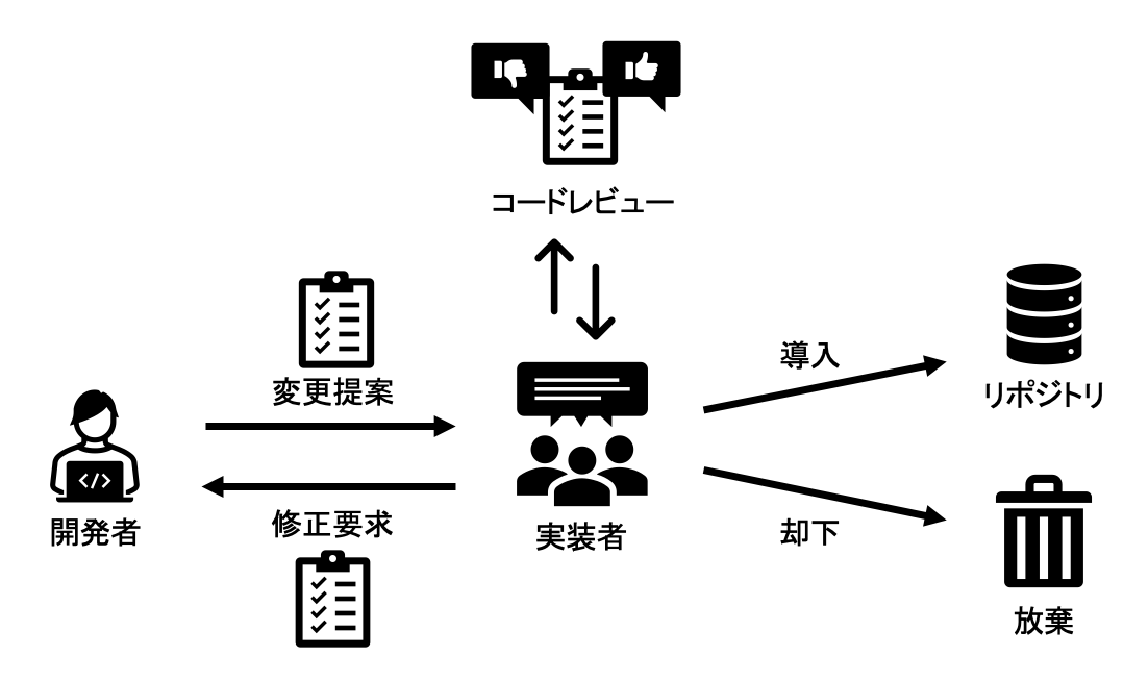
\includegraphics[width=1.0\linewidth]{Uenaka_fig/code_review_process.pdf}
\caption{コードレビュープロセス}
\label{fig:codereviewprocess}
\end{center}
\end{figure}
%-----------------------

\subsection{従来研究}

\subsubsection{変更提案の優先順位付け}
従来研究では,OSS開発を対象にコードレビューのための変更提案の優先順位付け手法を提案している.従来研究では,機械学習アルゴリズムを用いて,変更内容や作成者の特徴などの14種類の特徴を説明変数とし,翌日までに検証される否かを予測する手法を提案している\cite{prioritizer}.機械学習モデルの性能評価のために,475プロジェクトに適用した結果,適合率0.64,再現率0.85を達成している.

%¥begin{table}[t]
%  ¥caption{従来研究¥cite{prioritizer}で用いる14種類の説明変数}
%  ¥label{table:juurai}
%  ¥centering
%  ¥vspace{0.5zh}
%  ¥begin{tabular}{l|lr}
%    ¥hline
%    ¥multicolumn{1}{c|}{説明変数}  & ¥multicolumn{1}{|c}{説明}  ¥¥
%    ¥hline ¥hline
%    経過時間  & 変更提案が提出されてからの経過分数 ¥¥
%    貢献率  & 変更提案作成者のプロジェクトでのコミット率 ¥¥
%    受入率  & 変更提案作成者が過去に提出した変更提案の導入率 ¥¥
%    追加行数  &  変更提案で追加されている変更行数 ¥¥
%    削除行数  & 変更提案で削除されている変更行数  ¥¥
%    リビジョン数  & 変更提案のリビジョン数 ¥¥
%    ファイル数  & 変更提案の変更ファイル数 ¥¥
%    コメント数 & 変更提案のコメント数 ¥¥
%    レビュー数  &  変更提案に対してのコードレビュー数 ¥¥
%    コアメンバー  & 変更提案の作者はプロジェクトメンバーか ¥¥
%    ブランチ  & 変更コードとマージ先のリポジトリが同一か ¥¥
%    issue含有  & 変更提案に紐づいているissueがあるか ¥¥
%    最終コメント &  最終コメントでユーザがメンションされているか ¥¥
%    テストコード含有  & 変更ファイルにテストコードが含まれているか ¥¥
%    ¥hline
%  ¥end{tabular}
%¥end{table}


\subsubsection{変更提案の導入と開発者間の関係}
Bosu\cite{review1}らは,OSS開発における開発者の地位が変更提案の導入に影響するのか否かを明らかにするために,OSS開発を活発に行う開発者と不活発な開発者での変更提案の導入プロセスの違いに関する調査を行なった.8つのOSSプロジェクトから導入もしくは却下と判断された変更提案のコードレビューデータを調査した結果,変更提案は,積極的に貢献する開発者の依頼ほど,導入もしくは却下までの時間が短く,導入される確率が高いことが明らかとなった.そのため本論文では,開発で導入される変更提案の予測モデル構築の際に,初回のコードレビューが行われるまでの時間や,初回のコードレビューが行われてからの時間を特徴量として学習させることで,予測精度の向上を図る.



%¥subsection{動機}
%従来研究¥cite{prioritizer}では,ソフトウェア開発において優先的にコードレビューを行う変更提案の選択を容易にするために,変更提案に対して優先順位付けを行なっているが,変更提案の特徴量のみを用いて予測を行うため,直近のバージョンリリースまでの期間やその時点での対応可能な開発者数などの開発状況は考慮されていない.しかし,ソフトウェア開発において,バージョンリリースが近い場合は新たに提出された大規模な変更を導入するためにコードレビューのリソースを割く時間が無いというように,開発状況によって対応する変更提案は異なると考える.RQでは,リリースまでの期間に応じた変更提案の導入に重要な特徴を調査する.

%¥section{リサーチクエスチョン}
%本論文では,2つのRQを設定し,検証することで本研究の選択手法が直近のバージョンリリースに導入される変更提案の選択に有効かを評価する.
% ¥begin{itemize}
%  ¥item RQ1:リリースまでの期間に応じて優先的に導入される変更提案の特徴は異なるか?
%  ¥item RQ2:開発状況を考慮した変更提案の選択手法は直近のバージョンリリースに導入される変更提案をどの程度選択するか?
% ¥end{itemize}
% 
% RQ1では,リリースまでの期間に応じた変更提案の導入に重要な特徴の調査を行う.RQ2では,ナップサック問題を用いて変更提案の選択手法を定式化し,実際に行われた開発と比較することで,実際の開発で導入された変更提案をどの程度選択するかの調査を行う.
 
 
\section{分析対象データセット}\label{chap:dataset}

本研究では,OpenStackにおけるプロジェクトの中からコアコンポーネントを構築するNova,Neutron,Cinder,Keystone,Swift,Glanceの6プロジェクトを分析対象とする.各プロジェクトの変更提案の中から,2023年1月時点で導入もしくは却下されることが決定している変更提案を収集する.具体的には,OpenStackがコードレビュー管理システムとして使用するGerrit\footnote{Gerrit: \url{https://review.opendev.org}}から,変更提案のリビジョンごとの特徴量や,コードレビュー履歴を収集し,GitHubから,プロジェクトのコミット履歴や,リリースバージョンのリリース日やコミットハッシュを収集した.それぞれのプロジェクトの変更提案数は表\ref{table:release}のプロジェクト名の下に示す.また,表\ref{table:release}には,各プロジェクトにおいてリリースされたバージョンと,導入された変更提案数の上位5バージョンを示す.本研究では,正解ラベルのついた変更提案数を一定以上確保するためにこれら5バージョンを分析対象とする.

\begin{table}[t]
\centering
  \caption{プロジェクトごとの変更提案数}
  \vspace{0.5zh}
  \label{table:henkou}
  \begin{tabular}{l|r}  \hline
    \multicolumn{1}{c|}{プロジェクト} & \multicolumn{1}{|c}{変更提案数} \\ \hline \hline
    Neutron & 24,467 \\ \hline
    Keystone & 10,764 \\ \hline
    Horizon & 12,475 \\ \hline
    Nova & 39,870 \\ \hline
  \end{tabular}
\end{table}

\begin{table}[t]
\centering
  \caption{プロジェクトごとの対象リリースバージョン}
  \vspace{0.5zh}
  \label{table:release}
  \scalebox{0.75}{
  \begin{tabular}{l|ll|c}  \hline
    \multicolumn{1}{c|}{プロジェクト} & \multicolumn{1}{|c}{リリースバージョン(変更提案数 )}\\ \hline \hline
    Neutron  & 2013.1.g3(317),2013.2.b2(580),2013.2.rc1(423),2014.2.b1(320),\\ 
   (24,467) 	& 2015.1.0b1(391),2015.1.0b2(306),7.0.0.0b1(371),7.0.0.0b3(396),\\ 
	& 8.0.0.0b1(408),8.0.0.0b2(326),9.0.0.0b3(363),11.0.0.0b3(388),\\ 
	& 15.0.0.0b1(312),19.0.0.0rc1(420),20.0.0.0rc1(380) \\ \hline
%    Keystone  & 2011.3(195),essex-4(357),2013.2.b1(186),2013.2.b3(261),¥¥
%    (10,764) & 2014.1.b3(252),2014.2.b1(185),2015.1.0rc1(199),8.0.0a0(187),¥¥ 
%     & 9.0.0.0b2(212),9.0.0.0b3(214),10.0.0.0b1(179),10.0.0.0b2(220),¥¥ 
%     & 11.0.0.0b1(273),15.0.0.0rc1(408),16.0.0.0rc1(225) ¥¥ ¥hline
%    Horizon  & folsom-2(391),2014.2.b2(190),2014.2.b3(279),2015.1.0b2(198),¥¥
%    (12,475) & 2015.1.0b3(237),8.0.0.0b2(402),8.0.0.0b3(384),9.0.0.0b1(230),¥¥
%      & 9.0.0.0b3(237),10.0.0.0b2(193),10.0.0.0b3(171),11.0.0.0b2(193),¥¥
%       & 13.0.0.0b1(310),14.0.0.0b1(194),15.0.0.0b2(178) ¥¥ ¥hline
    Nova & folsom-1(1,550),2013.1.rc1(2723),2013.2.b3(1,517),2013.2.rc1(555),\\ 
   (39,870)  & 2014.1.b3(517),2014.2.b2(554),2015.1.0b2(838),2015.1.0b3(625),\\
     & 13.0.0.0b3(529),14.0.0.0b2(607),16.0.0.0b2(524),17.0.0.0b1(516),\\ 
     &19.0.0.0rc1(865),21.0.0.0rc1(808),24.0.0.0rc1(771) \\ \hline
  \end{tabular}
  }
\end{table}


\section{RQ1:\rqone}\label{chap:rq-1}

\subsection{概要}
直近のリリースまでの期間などの開発状況によって,直近のリリースに導入される変更提案の優先順位は異なることが示唆される.RQ1では,直近のリリースまでの期間に応じてコードレビューに取り組まれる変更提案の特徴は異なるのかを明らかにする.
%各プロジェクトにおける変更提案のタイトルと概要に含まれる単語の異なる変更提案間での頻度をリリースまでの期間ごとに調査し,比較する.

\subsection{分析手法}

\subsubsection{変更提案内容の分析方法}
RQ1では,変更提案の特徴を理解するために,変更提案を説明する自然言語で記述された内容を調査する.本RQでは,分析対象とするOpenStackが使用するGerritにおいて,変更提案の説明として各チケットに含まれるタイトルと概要を分析する.具体的には,説明に含まれる名詞,形容詞,動詞の単語出現頻度を分析する.本節で単語出現頻度分析のために次の手順で前処理を行う.

\begin{enumerate}
  \item{\textbf{記号等の削除:}}
  タイトル・概要に含まれる記号と数字,空白を削除する.
  \item{\textbf{小文字統一:}}
  単語の大文字を小文字に変換することで,全て小文字表記に統一する.
  \item{\textbf{ストップワードの除去:}}
  記号等を削除したタイトルと概要から,前置詞や助動詞,接続詞や冠詞,代名詞の除去を行う.除去対象とする単語はPythonのnltk.corpus.stopwordsに含まれる単語に基づく.
  \item{\textbf{ノイズとなる単語の削除:}}  
  変更提案の概要に必ず含まれる「commit-id」のように,変更提案の特徴が反映されないかつ複数のタイトル・概要に含まれる単語を,ノイズとなる単語として複数削除する.
  \item{\textbf{表記の統一:}}
  単語ごとに語幹の統一を行う.この処理にはPythonのnltk.stem.porterのstemモジュールを利用する.
\end{enumerate}

\subsubsection{リリースまでの期間ごとの単語の頻度分析}
直近のリリースまでの期間に応じた変更提案の特徴の違いを明らかにするために,リリースまでの期間として1週間前,2週間前,1ヶ月前,2ヶ月前の4時点を分析対象期間とし,リリースまでの期間に応じた単語の頻度の違いを,2種類の比較方法で分析する.

\begin{enumerate}
  \item{\textbf{コードレビューに取り組まれた変更提案と取り組まれなかった変更提案:}}
  レビュー対象とする変更提案の特徴がリリースまでの期間ごとにどのように異なるのかを比較する.
  \item{\textbf{コードレビューに取り組まれた変更提案のうち,直近のリリースに導入された変更提案と導入されなかった変更提案:}}
  レビュー対象とする変更提案のうち,直近のリリースに導入される変更提案の特徴がリリースまでの期間ごとにどのように異なるのかを比較する.
\end{enumerate}

\subsection{分析結果}

\section{おわりに}\label{chap:fig-tab-exp}
%%%%%%%%%%%%%%%%

本論文では,直近のバージョンリリースに導入される変更提案の選択を容易にすることを目的として,開発状況を考慮した変更提案の選択手法を提案し,設定したRQを検証した.対象データセットとして,OpenStackにおけるプロジェクトの中から,膨大な変更提案が提出されているNeutron,Keystone,Horizon,Novaプロジェクトの変更提案を収集し,変更提案の特徴量を学習させることで,直近のバージョンリリースに導入される変更提案の予測モデルを構築した.モデルの予測精度を評価した結果,MAEやRMSEが高い精度であった一方,決定係数の値は低くなるという結果が得られた.また,予測の際に重要となった特徴を確認した結果,リリースが遠い時点では初回のレビューからの経過時間が重要となるが,リリースが近づくにつれて作成からの経過時間が重要となった.

\textbf{謝辞}\
本フォーマットの基になったスタイルファイルを作成してくださった方々に感謝します.

%\begin{adjustvboxheight} % needed only when Appendix follows
%\bibliographystyle{jssst}
%\bibliography{sample}
%\end{adjustvboxheight} % needed only when Appendix follows

% 以下はbibtexを使用しない場合の例です.
% 332行目と333行目をコメントアウトしてから使用してください.
% なお,この例では年数順に文献が並んでいるので適切な並び順ではありません.
%\begin{adjustvboxheight} % needed only when Appendix follows
%\begin{thebibliography}{9}
%\bibitem{fose2016} 阿萬 裕久,横川 智教 編:ソフトウェア工学の基礎XXIII,日本ソフトウェア科学会{\em FOSE2016}, 近代科学社, 2016.
%\bibitem{fose2017} 吉田 敦,福安 直樹 編:ソフトウェア工学の基礎XXIV,日本ソフトウェア科学会{\em FOSE2017}, 近代科学社, 2017.
%\bibitem{fose2018} 伊藤 恵,神谷 年洋 編:ソフトウェア工学の基礎XXV,日本ソフトウェア科学会{\em FOSE2019}, 近代科学社, 2018. 
%\bibitem{fose2019} 森崎修司,大平雅雄 編:ソフトウェア工学の基礎XXVI,日本ソフトウェア科学会{\em FOSE2019}, 近代科学社, 2019. 
%\bibitem{fose2020} 石尾 隆,天嵜 聡介 編:ソフトウェア工学の基礎XXVII,日本ソフトウェア科学会{\em FOSE2020}, 近代科学社, 2020. 
%\bibitem{fose2021} 名倉 正剛,関澤 俊弦 編:ソフトウェア工学の基礎28,日本ソフトウェア科学会{\em FOSE2021}, 近代科学社, 2021.
%\bibitem{fose2022} 角田 雅照,まつ本 真佑 編:ソフトウェア工学の基礎29,日本ソフトウェア科学会{\em FOSE2022}, 近代科学社, 2022.
%\bibitem{fose2023} 吉田 則裕,槇原 絵里奈 編:ソフトウェア工学の基礎30,日本ソフトウェア科学会{\em FOSE2023}, 近代科学社, 2023. 
%\bibitem{fose2024} 戸田 航史, 藤原 賢二 編:ソフトウェア工学の基礎31,日本ソフトウェア科学会{\em FOSE2024}, 近代科学社, 2024. (to appear)
%\end{thebibliography}
%\end{adjustvboxheight} % needed only when Appendix follows

%以下は付録の例です.必要ならコメントアウトして使用してください.
%なお,その際には参考文献の前後にある adjustvboxheight 環境のコメントアウトを解除してください.
%\appendix
%\section{付録A} 
%これは付録の例です.

\bibliographystyle{plain}
\bibliography{Uenaka}

\end{document}

